\documentclass[10pt]{article}

% amsmath package, useful for mathematical formulas
\usepackage{amsmath}
% amssymb package, useful for mathematical symbols
\usepackage{amssymb}

% graphicx package, useful for including eps and pdf graphics
% include graphics with the command \includegraphics
\usepackage{graphicx}

% cite package, to clean up citations in the main text. Do not remove.
\usepackage{cite}

\usepackage{color} 

% Use doublespacing - comment out for single spacing
\usepackage{setspace} 
\doublespacing


% Use the PLoS provided bibtex style
\bibliographystyle{PLoS2009}

% Remove brackets from numbering in List of References
\makeatletter
\renewcommand{\@biblabel}[1]{\quad#1.}
\makeatother


% Leave date blank
\date{}

\pagestyle{myheadings}
%% ** EDIT HERE **
%% Please insert a running head of 30 characters or less.  
%% Include it twice, once between each set of braces
\markboth{Nanopore automata}{Nanopore automata}


%% ** EDIT HERE **
%% PLEASE INCLUDE ALL MACROS BELOW

\usepackage{setspace}
\doublespacing



\newcommand\titlestring{Nanopore automata}
\newcommand\authorstring{
Ian Holmes$^{1,2,\ast}$
\\
\textbf{1} Lawrence Berkeley National Laboratory, Berkeley, CA, USA
\\
\textbf{2} Department of Bioengineering, University of California, Berkeley, CA, USA
}

\usepackage{array}


% Labels & references for sections, figures and tables
% Comment out \secref and \seclabel for PLoS, which doesn't like numbered section references
\newcommand{\secref}[1]{Section~\ref{sec:#1}}
\newcommand{\seclabel}[1]{\label{sec:#1}}
\newcommand{\secname}[1]{``#1''}  % PLoS-style section names

% "Text S1", "Text S2", etc.
\newcommand{\supptext}[1]{Text S#1}

% "Dataset S1", "Dataset S2", etc.
\newcommand{\dataset}[1]{Dataset S#1}

% Appendix
\newcommand{\appref}[1]{Appendix~\ref{app:#1}}
\newcommand{\applabel}[1]{\label{app:#1}}

% Figure
\newcommand{\figref}[1]{Figure~\ref{fig:#1}}
\newcommand{\figlabel}[1]{\label{fig:#1}}

% Table
\newcommand{\tabnum}[1]{\ref{tab:#1}}
\newcommand{\tabref}[1]{Table~\tabnum{#1}}
\newcommand{\tablabel}[1]{\label{tab:#1}}

% Equation
\newcommand{\eqnref}[1]{Equation~\ref{eqn:#1}}
\newcommand{\eqnlabel}[1]{\label{eqn:#1}}


% need cite, check me, and other notes to self
\newcommand\needcite{{\bf [CITE]}}
\newcommand\checkme{{\bf [CHECK]}}

% indicator function
\newcommand\indicator[1]{\delta\left(#1\right)}

% Probability
\newcommand\prob[1]{\mbox{Pr} \left[ #1 \right]}

%% END MACROS SECTION

\begin{document}

% Title must be 150 words or less
\begin{flushleft}
  {\Large
    \textbf{\titlestring}
  }
\\
\authorstring
\end{flushleft}


% Table of contents
\tableofcontents


% Please keep the abstract between 250 and 300 words
%\newpage
\section{Abstract}
State machine algorithms for aligning Nanopore reads.

% Please keep the Author Summary between 150 and 200 words
% Use first person. PLoS ONE authors please skip this step. 
% Author Summary not valid for PLoS ONE submissions.   
%\newpage
%\section{Author Summary}


%\newpage
%\section{Introduction}

%\newpage
\section{Specification}

Initial goal (Preliminary Results) is simple reusable code for aligning a segmented nanopore read (with segment currents summarized) to a reference sequence.

Longer-term goals (Specific Aims) include
\begin{itemize}
\item quasi-hierarchical series of models for processed$\to$raw data (raw, FAST5, FASTQ, FASTA)
\item transducer intersection-style models for read-pair alignment
\item systematic strategies for approximation/optimization algorithms, climbing the hierarchy (starting with k-mer or FM-index approaches)
\item transducer intersection models for aligning reads from different sequencing technologies
\end{itemize}

\subsection{Parameterization algorithm}

Given the following inputs
\begin{itemize}
\item Reference genome (FASTA)
\item Segment-called reads (FAST5/HDF5)
\end{itemize}

Perform the following steps
\begin{itemize}
\item Perform Baum-Welch to fit a rich model
\end{itemize}

Rich model incorporates segment statistics.

\subsection{Reference search algorithm}

Given the following inputs
\begin{itemize}
\item Reference genome
\item Segment-called reads (FAST5/HDF5)
\item Parameterized rich model
\end{itemize}

Perform the following steps
\begin{itemize}
\item Perform Viterbi alignment
\end{itemize}

\subsection{Implementation}

Libraries etc.

HDF5...

\subsection{Evaluation}

Strategy...

Data sets...

\section{Methods}

Model \& inference algorithms.

\subsection{Model}

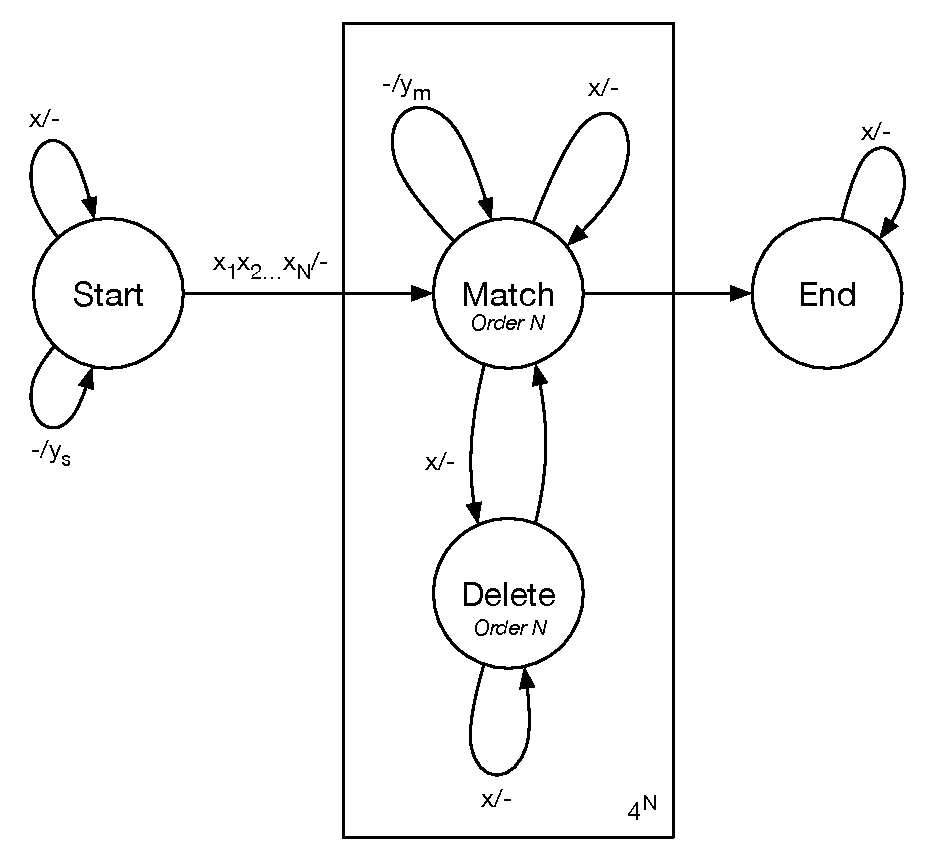
\includegraphics[width=\textwidth]{figs/Transducer.pdf}

\newcommand\paramlabel[1]{\mbox{\tiny #1}}

\begin{itemize}
\item Order-$N$ transducer.
\item Input alphabet: $\Omega = \{ A, C, G, T \}$ (nucleotides)
\item Output alphabet: $\Re$ (real numbers signifying current levels)
\item States: Start, Match${}_{x_1 \ldots x_N}$, Delete${}_{x_1 \ldots x_N}$, End
\item Parameters:
$p^{\paramlabel{StartEmit}}, p^{\paramlabel{BeginDelete}}, p^{\paramlabel{ExtendDelete}}, \mu^{\paramlabel{Start}},\tau^{\paramlabel{Start}},$ \\
$\{ p^{\paramlabel{MatchEmit}}_{x_1\ldots x_N}, \mu^{\paramlabel{Match}}_{x_1\ldots x_N},\tau^{\paramlabel{Match}}_{x_1\ldots x_N} : x_1 \ldots x_N \in \Omega^N \}$
\end{itemize}

\noindent Transitions:
\\
\noindent
\begin{tabular}{lllll}
\hline
Source & Destination & Weight & Absorbs & Emits \\
\hline
Start & Start & $p^{\paramlabel{StartEmit}}$ & & $y_s \sim \mbox{Normal}(\mu^{\paramlabel{Start}},\tau^{\paramlabel{Start}})$ \\
& & $\times P(y_s|\mu^{\paramlabel{Start}},\tau^{\paramlabel{Start}})$ & & \\
Start & Start & $1$ & $x \in \Omega$ & \\
Start & Match${}_{x_1 \ldots x_N}$ & $1 - p^{\paramlabel{StartEmit}}$ & $x_1 \ldots x_N \in \Omega^N$ & \\
Match${}_{x_1 \ldots x_N}$ & Match${}_{x_1 \ldots x_N}$ & ${p^{\paramlabel{MatchEmit}}_{x_1\ldots x_N}}$ & & $y_m \sim \mbox{Normal}(\mu^{\paramlabel{Match}}_{x_1\ldots x_N},\tau^{\paramlabel{Match}}_{x_1\ldots x_N})$ \\
& & $\times P(y_m|\mu^{\paramlabel{Match}}_{x_1\ldots x_N},\tau^{\paramlabel{Match}}_{x_1\ldots x_N})$ & & \\
Match${}_{x_1 \ldots x_N}$ & Match${}_{x_2 \ldots x_{N+1}}$ & $(1 - {p^{\paramlabel{MatchEmit}}_{x_1\ldots x_N}})$ & $x_{N+1} \in \Omega$ & \\
& & $\times (1 - p^{\paramlabel{BeginDelete}})$ & & \\
Match${}_{x_1 \ldots x_N}$ & Delete${}_{x_2 \ldots x_{N+1}}$ & $(1 - {p^{\paramlabel{MatchEmit}}_{x_1\ldots x_N}})$ & $x_{N+1} \in \Omega$ & \\
& & $\times p^{\paramlabel{BeginDelete}}$ & & \\
Match${}_{x_1 \ldots x_N}$ & End & $1 - {p^{\paramlabel{MatchEmit}}_{x_1\ldots x_N}}$ & & \\
Delete${}_{x_1 \ldots x_N}$ & Delete${}_{x_2 \ldots x_{N+1}}$ & $p^{\paramlabel{ExtendDelete}}$ & $x_{N+1} \in \Omega$ & \\
Delete${}_{x_1 \ldots x_N}$ & Match${}_{x_1 \ldots x_N}$ & $1 - p^{\paramlabel{ExtendDelete}}$ & & \\
End & End & 1 & $x \in \Omega$ & \\
\hline
\end{tabular}




\subsection{Baum-Welch algorithm}

As usual.

\subsection{Viterbi algorithm}

As usual.


% Results and Discussion can be combined.
\newpage
\section{Results}




\section{Discussion}


% Do NOT remove this, even if you are not including acknowledgments
\newpage
\section{Acknowledgments}

%\section{References}
% The bibtex filename
\bibliography{../latex-inputs/alignment,../latex-inputs/reconstruction,../latex-inputs/duplication,../latex-inputs/genomics,../latex-inputs/ncrna,../latex-inputs/url}

\clearpage
\section{Figure Legends}

\clearpage
\section{Appendix}

\subsection{Exponential distribution}

\begin{eqnarray*}
x & \sim & \mbox{Exponential}(\kappa) \\
P(x|\kappa) & = & \kappa \exp(-\kappa x) \\
\mbox{E}[x] & = & \kappa^{-1} \\
\mbox{Var}[x] & = & \kappa^{-2}
\end{eqnarray*}

Rate parameter $\kappa$.


\subsection{Gamma distribution}

\begin{eqnarray*}
x & \sim & \mbox{Gamma}(\alpha,\beta) \\
P(x|\alpha,\beta) & = & \frac{x^{\alpha-1} \beta^\alpha \exp(-x \beta)}{\Gamma(\alpha)} \\
\mbox{E}[x] & = & \alpha/\beta \\
\mbox{Var}[x] & = & \alpha/\beta^2
\end{eqnarray*}

Shape parameter $\alpha$, rate parameter $\beta$.
$\Gamma()$ is the gamma function
\[
\Gamma(\alpha) = \int_0^{\infty} z^{\alpha-1} \exp(-z) dz
\]
Note $\Gamma(n) = (n-1)!$ for positive integer $n$.

\subsection{Normal distribution}

\begin{eqnarray*}
x \sim \mbox{Normal}(\mu,\tau)
\end{eqnarray*}


Mean $\mu$, precision $\tau$ (precision is reciprocal of variance).
\[
P(x|\mu,\tau)
 = \sqrt{\frac{\tau}{2\pi}} \exp \left( -\frac{\tau}{2}(x-\mu)^2 \right)
\]


\end{document}

